
	This chapter covers the required theoretical background and consists 
	of the following main parts:

	\begin{enumerate}
		\item Graph Theory
		\item Machine Learning on Graphs
		\item Graph Generation
    \end{enumerate}

	\section{Graph Theory}

	This section provides a brief introduction to graph theory with a focus on
	the relevant aspects for this master's thesis. The theory presented in this
	section is primarily taken from the book "Networks: An Introduction" by 
	Mark Newman \citeyearpar{Newman2010}. \\

	\noindent Graph theory is an old field of mathematics and can be traced back 
	to Leonhard Euler and the famous "Königsberg Bridge Problem"
	\citep{euler1741solutio}. The study of graphs has had a recent revival
	thanks to its useful applications in areas such as the Google algorithm
	PageRank \citep{page1999pagerank} and graph machine learning. Graphs are 
	special data structures for which an example is shown in Figure 
	\ref{fig:graph}. The terms graph and network are often used interchangeably 
	and have the identical meaning for the purpose of this master's thesis. 
	Typically, the term graph is used more commonly for the mathematical 
	analysis of graphs and the term network is more commonly used in data
	science.  

	\begin{figure}[h]
		\centering
		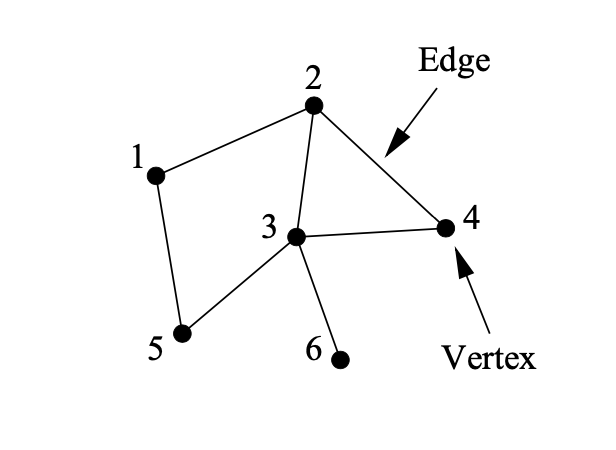
\includegraphics[width=0.5\textwidth]{graph.png}
		\caption{Example of a Graph}
		\cite[p. 111]{Newman2010}
		\label{fig:graph}
	\end{figure}
	
	\noindent The graph shown in Figure \ref{fig:graph} corresponds to an 
	undirected graph in which the connections between the vertices are mutual. 
	In a directed graph for instance, vertex A could be connected to vertex B, 
	however vertex B need not be connected to vertex A. For the purpose of this 
	thesis, only undirected graphs are considered. Vertices are often referred 
	to as nodes and the terms are used interchangeably. Edges refer to the
	connections between the vertices. The term links is also often used to
	refer to edges and the terms are used interchangeably as well. Graphs may have 
	additional elements such as multi-edges or self-edges. Self-edges refer to
	nodes which have a looped link to themselves. This can be considered as a
	form of feedback loop of a node on to itself. Lastly, multi-edges refer to 
	direct node connections with multiple paths. For notation purposes, graphs 
	are typically defined as follows:

	\begin{equation}
		G(V,E)
	\end{equation}

	\noindent $G$ denotes the graph, $V$ refers to the set of vertices present 
	in the graph, and $E$ refers to edges present between the vertices. \\

	\noindent This concludes the basic setup of graphs. The following 
	paragraphs give an introduction to the adjacency matrix, node degrees, and 
	centrality measures which are used in this thesis.

	\paragraph{Adjacency Matrix} \mbox{}\\  

	\noindent The adjacency matrix $A$ is defined as a $n \times n$ matrix, 
	where $n$ refers to the number of vertices present in the graph. Each 
	vertex is therefore recorded by a column and a row in the adjacency matrix. 
	The elements in the adjacency matrix are further typically defined as follows:

	\begin{equation}
		A_{ij} = 
			\begin{cases}
				1, & \text{if vertex $i$ and $j$ are connected by an edge} \\
				0, & \text{otherwise}
			\end{cases}
	\end{equation}
	
	\noindent For illustration, the adjacency matrix of the graph depicted in 
	Figure \ref{fig:graph} is shown as follows:

	\[ A = 
	\begin{pmatrix}
		0 & 1 & 0 & 0 & 1 & 0 \\
		1 & 0 & 1 & 1 & 0 & 0 \\
		0 & 1 & 0 & 1 & 1 & 1 \\
		0 & 1 & 1 & 0 & 0 & 0 \\
		1 & 0 & 1 & 0 & 0 & 0 \\
		0 & 0 & 1 & 0 & 0 & 0  
	\end{pmatrix}
	\] 
	
	\noindent As one can see in the adjacency matrix, if vertex $i$ and $j$ are 
	connected, this is recorded with 1 and 0 otherwise. Note, that all of the 
	elements on the $diag(A)$ are equal to 0. This is because there are no 
	self-edges present in figure \ref{fig:graph}. Nodes with self-loops would 
	have a 1 recorded on the corresponding diagonal element of the adjacency 
	matrix. In addition, multi-edges can be recorded with the number of edges
	present between two vertices. For example, vertices which are connected by
	two edges would be recorded with a 2 in the adjacency matrix. The graph
	shown in figure \ref{fig:graph} is an undirected network. For that reason, 
	the adjacency matrix is symmetric. The adjacency matrix can further be used 
	for representing different types of graphs such as weighted networks. These 
	aspects are however not relevant for this thesis. For additional information 
	regarding the adjacency matrix, again the book by Mark Newman 
	\citeyearpar{Newman2010} is highly recommended. 

	\paragraph{Degree Measures} \mbox{}\\

	\noindent An important measure for graphs are the vertex degrees denoted by 
	$k$. Degrees refer to the number of edges connected to a vertex. The 
	degrees of vertex $i$ can be formulated as \citep[p. 133]{Newman2010}:

	\begin{equation}
		k_i = \sum_{j=1}^{n} A_{ij}
	\end{equation}

	\noindent For an undirected graph, edges have two ends. This is due to the 
	fact, that vertices connected by an edge are mutually connected. To
	calculate the sum of the degrees of all vertices, one can therefore write 
	for an undirected graph with $m$ edges and $n$ vertices 
	\citep[p. 133]{Newman2010}:

	\begin{equation}
		2m = \sum_{i=1}^{n} k_i	
	\end{equation}

	\noindent As a statistical measure, the mean degree $c$ of a vertex is 
	defined as follows \citep[p. 134]{Newman2010}:

	\begin{equation}
		c = \frac{1}{n}\sum_{i=1}^{n}k_i = \frac{2m}{n}
	\end{equation}

	\noindent To calculate the density of a graph, it should first be noted, 
	that the maximum number of edges is given by \citep[p. 134]{Newman2010}:

	\begin{equation}
		{n \choose 2} = \frac{1}{2}n(n-1)
	\end{equation}

	\noindent The density $\rho$ can thus be written as \citep[p. 134]{Newman2010}:

	\begin{equation}
		\rho = \frac{m}{{n \choose 2}} = \frac{2m}{n(n-1)} = \frac{c}{n-1}
	\end{equation}

	\noindent Note, that the density $\rho$ lies strictly between 
	$0 \leqslant \rho \leqslant 1$. In addition, for sufficiently large graphs,
	one can approximate $\rho = \frac{c}{n}$. 

	\paragraph{Eigenvector Centrality} \mbox{}\\

	\noindent The degrees of a vertex shown in the previous section correspond 
	to the simplest form of a centrality measure. The issue with this measure 
	is, that the every neighbor of vertex $i$ is valued the same. This is a 
	problem, as not all neighbors are of equal importance due to:

	\begin{enumerate}
		\item The number of the neighbor's neighbors
		\item The importance of the neighbor
		\item Both
	\end{enumerate}

	\noindent There are many different alternative centrality measures which
	can consider the factors listed above such as eigenvector centrality, Katz
	centrality, and PageRank
	\citep{landau1895relativen,katz1953new,page1999pagerank}. For analyzing 
	undirected graphs, eigenvector centrality is sufficient and is presented in 
	more detail.\\

	\noindent Eigenvector centrality gives all vertices a centrality score which 
	is proportional to the sum of the scores of the vertices' neighbors. This is 
	a procedure in which typically the initial centrality $x_i$ of vertex $i$ is 
	guessed to be 1, $\forall i$. This can be used to calculate the 
	centralities of the neighbors of $i$ which is denoted as $x_{i}'$. One can 
	thus write \citep[p. 169]{Newman2010}:

	\begin{equation}
		x_i' = \sum_{j}A_{ij}x_j
	\end{equation}
	\newpage
	\noindent In matrix notation:

	\begin{equation}
		x' = Ax
	\end{equation}

	\noindent This process is repeated $t$ times as follows to generate better 
	estimates \citep[p. 170]{Newman2010}:

	\begin{equation}
		x(t) =  A^tx(0)
	\end{equation}

	\noindent Where $x(0)$ denotes the linear combination of 
	\citep[p. 170]{Newman2010}:

	\begin{equation}
		x(0) =  \sum_{i}c_{i}v_{i}
	\end{equation}

	\noindent The variable $v_i$ denotes the eigenvectors of the adjacency 
	matrix $A$ and $c_i$ corresponds to an appropriately chosen constant. 
	Therefore one can write \citep[p. 170]{Newman2010}:

	\begin{equation}
		x(t) =  A^t \sum_{i}c_{i}v_{i} = \sum_{i} c_i k_i^t v_i = 
		k_i^t \sum_{i} c_i \left[\frac{k_i}{k_1}\right]^t v_i
		\label{eq:eigenvec_cent}
	\end{equation}

	\noindent In equation \ref{eq:eigenvec_cent}, $k_i$ correspond to the 
	eigenvalues of the adjacency matrix $A$. $k_1$ corresponds to the largest 
	eigenvalue of $A$. As $\frac{k_i}{k_1} < 1, \; \forall \; i\neq 1$ , the 
	term is decaying as $t \rightarrow \infty$. The centralities $x$ can 
	therefore be written in terms of fulfilling following condition 
	\citep[p. 170]{Newman2010}:

	\begin{equation}
		Ax = k_1 x	
	\end{equation}

	\noindent Thus, the eigenvector centrality is defined as 
	\citep[p. 170]{Newman2010}:

	\begin{equation}
		x_i = k_{1}^{-1} \sum_{j} A_{ij}x_j 
	\end{equation}

	\paragraph{Closeness Centrality} \mbox{}\\

	\noindent The closeness centrality $C_i$ of vertex $i$ is defined as the 
	average distance to the other vertices in the graph. This centrality 
	measure is defined as follows \citep[p. 182]{Newman2010}:

	\begin{equation}
		C_i = \frac{1}{l_i} = \frac{n}{\sum_{j}d_{ij}}
	\end{equation}

	\noindent For this measure, central vertices exhibit high closeness 
	centrality and are therefore more closely connected to the other vertices 
	compared to vertices with low closeness centrality. The variable $l_i$
	denotes the average geodesic distance $d_{ij}$ of vertex $i$. The range of
	the closeness centrality lies within the range $0\leqslant
	C_{i}\leqslant1$.

	\paragraph{Betweenness Centrality} \mbox{}\\

	\noindent This centrality measures to which extent a vertex $i$ lies on 
	a geodesic path between two other vertices. For instance, a bottle neck 
	vertex would exhibit a large betweenness centrality if many nodes must pass 
	through it to reach their destination. More formally, betweenness 
	centrality $x_i$ is defined as \citep[p. 187]{Newman2010}:

	\begin{equation}
		x_i = \sum_{st} \frac{\eta_{st}^i}{g_{st}}
		\label{eq:between_cent}
	\end{equation}

	\noindent In equation \ref{eq:between_cent}, $\eta_{st}^i$ refers to the 
	number of geodesic paths from $s$ to $t$ which pass through vertex $i$. 
	Further, $g_{st}$ is defined as the number of geodesic paths between vertex 
	$s$ and $t$. \\

	\noindent In order to allow for a better comparison of betweenness
	centralities, it is often standardized by the number of connected vertex
	pairs $s$ and $t$ denoted by $\eta^2$. The betweenness centrality in its
	standardized form can thus be written as \citep[p.190]{Newman2010}:

	\begin{equation}
		x_i = \frac{1}{\eta^2}\sum_{st} \frac{\eta_{st}^i}{g_{st}}
	\end{equation}

	\noindent With this measure, the betweenness centrality is within the range
	$0\leqslant x_{i}\leqslant1$.

	\section{Machine Learning on Graphs}

	\noindent Graphs are special because the nodes/datapoints in a graph are 
	linked with each other. A practical example for this are social 
	networks. In a social network, the profiles of "Peter" and "Paul" might be 
	connected because "Peter" and "Paul" are friends. In addition, "Paul" and 
	"Peter" can only ever reach each other, if they are directly or perhaps 
	indirectly connected via a mutual friend. This aspect is unique to network 
	data and provides interesting additional information as well as added
	complexity. This property does not allow for comparing nodes in a graph
	using common distance measures such as Euclidean distances. The edges
	connecting the nodes only indicate that two nodes are connected. It
	however does not indicate whether two connected nodes are more- or less 
	similar compared to two other connected nodes. In addition, how similar are 
	indirectly connected nodes? Further, how similar or dissimilar are these 
	nodes compared to other indirectly connected nodes? This rapidly becomes a 
	very complex question. The challenge is thus to develop a model which can 
	accurately measure the similarities of the nodes present in a graph. 
	\acs{gml} provides solutions to this problem and can be grouped into the 
	following two main categories:

	\begin{enumerate}
		\item Graph representation learning
		\item Graph neural networks
	\end{enumerate}
	
	\noindent Graph representation learning refers to models which generate node
	embeddings of a given graph. Specifically, this approach creates vector 
	representations of the nodes in a graph given a defined similarity measure. 
	For these node vector representations, distance measures such as Euclidean 
	distances can be measured. The generated node embeddings can thus be used for
	downstream machine learning using standard machine learning models. A 
	\acs{gnn} can also generate node embeddings as well as directly using graphs 
	for a given classification task among others. The capability of
	directly applying graphs for machine learning, makes graph neural networks 
	especially promising. \\

	\noindent In the following subsections, the theory for \acs{grl} and
	\acsp{gnn} is introduced. 

	\subsection{Graph Representation Learning}

	The aim of \acf{grl} is to generate node embeddings in 
	the form of $d$-dimensional vector representations. The resulting node 
	embeddings can then be used for standard \acs{ml} applications. A graphical 
	representation of this task is shown in figure 
	\ref{fig:embedding}.

	\begin{figure}[h]
		\centering
		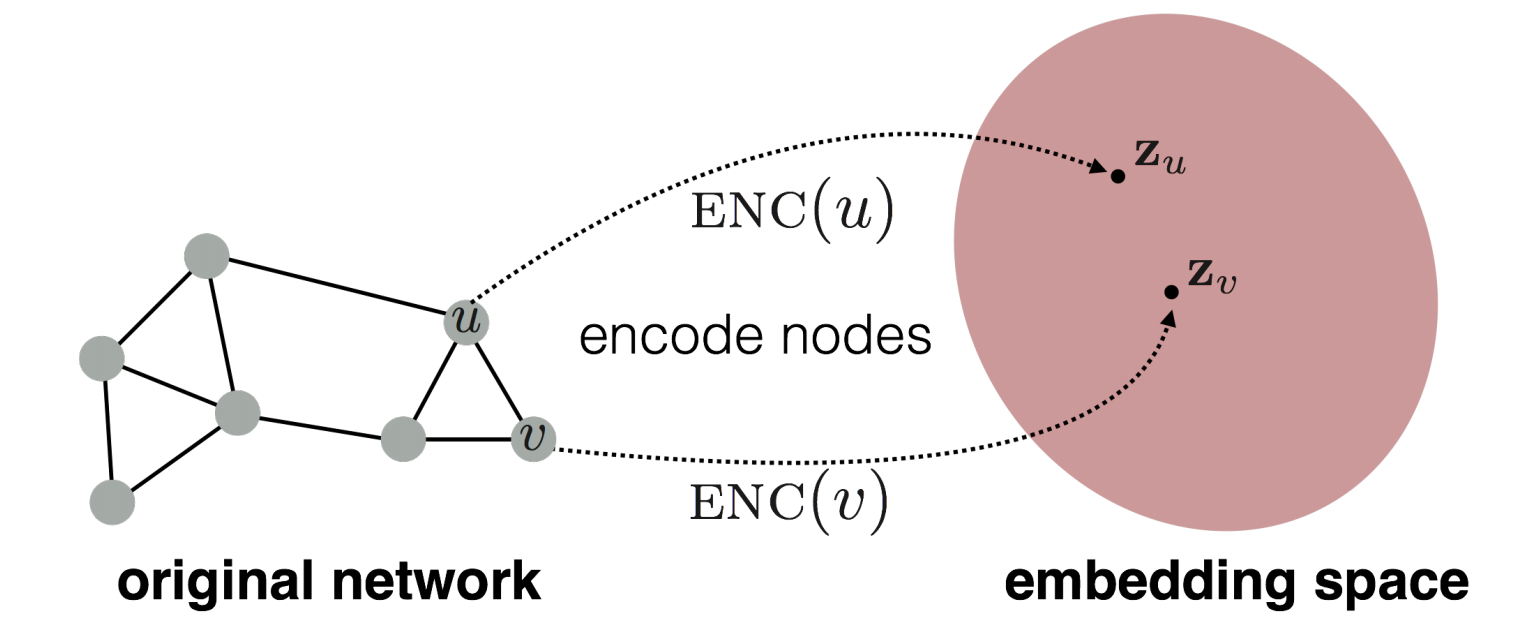
\includegraphics[width=0.8\textwidth]{embedding.png}
		\caption{Network Embedding}
		\cite{leskovec2021lecture}
		\label{fig:embedding}
	\end{figure}

	\noindent To generate node embeddings of a graph, one has to define an
	encoder which transforms nodes in a graph into their embedding space as
	shown in figure \ref{fig:embedding}. The nodes must be embedded in such a
	manner that similar nodes in the graph are also embedded closely in the 
	embedding space. A common measure for similarity is to find vector embeddings 
	$z$ of nodes $u$ and $v$ such that \citep{leskovec2021lecture}:

	\begin{equation}
		z_u^Tz_v \approx similarity(u,v)
		\label{eq:dot_sim}
	\end{equation}

	\noindent The dot product of the two node embedding vectors shown in
	equation \ref{eq:dot_sim} should thus approximately equal the similarity of 
	the corresponding nodes in the graph. There are different approaches for 
	defining node similarity. Graph factorization was introduced as an early 
	solution \citep{ahmed2013distributed}. More recent and successful approaches 
	include methods which make use of random walks. In the context of random 
	walks, similarity is defined as \citep{leskovec2021lecture}:

	\begin{equation}
		z_u^Tz_v \approx \text{Probability that node $u$ and $v$
								co-occur on a random walk over the graph}
	\label{eq:random_similartiy}
	\end{equation}

	\noindent The models DeepWalk \citep{perozzi2014deepwalk} and its 
	generalization Node2Vec \citep{grover2016node2vec} successfully apply the
	similarity measure shown in equation \ref{eq:random_similartiy}. Another 
	noteworthy model called LINE \citep{tang2015line} also makes use of random
	walk co-occurrences as its similarity measure. In order to remain focused,
	only DeepWalk and Node2Vec are considered for this thesis. These two models
	are well suited for the given task and are among the most popular \acs{grl} 
	models. \\

	\noindent DeepWalk and Node2Vec make use of methods which have its origin in 
	\ac{nlp}. Specifically they makes use of the Skip-gram model introduced by 
	\cite{mikolov2013efficient,mikolov2013distributed}. 
	The Skip-gram model is a core component of DeepWalk and Node2Vec, which is why 
	it is explained in detail before proceeding to the \acs{grl} models. \\

	\noindent In \ac{nlp} words are one-hot encoded as inputs for the Skip-gram 
	model which learns vector representations of the input words. The aim of the
	Skip-gram model is then to predict the context of the input word by
	predicting the neighboring words in a sentence. A basic overview of the 
	Skip-gram model is provided in figure \ref{fig:skip_gram}. 

	\begin{figure}[h]
		\centering
		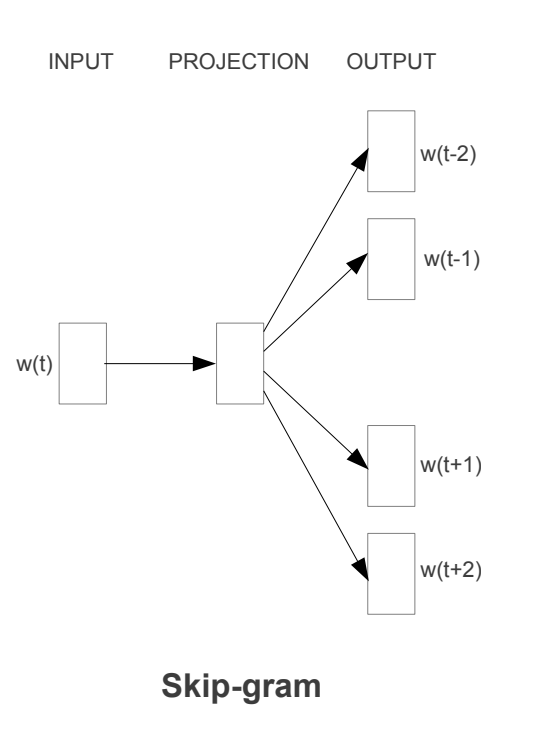
\includegraphics[width=0.4\textwidth]{skip_gram.png}
		\caption{Skip-gram Architecture}
		\cite[p. 5]{mikolov2013efficient}
		\label{fig:skip_gram}
	\end{figure}

	\noindent The basic layout shown in figure \ref{fig:skip_gram} depicts the
	high-level procedure of the Skip-gram model. To make this model more
	specific, the input corresponds to the one-hot encoded vector at row $t$ of
	the input matrix $W$ with dimensions $T \times T$, where every row 
	corresponds to a one-hot encoded word. $W(t)$ is linearly passed to the
	projection, which involves calculating the dot product of $W(t)$ with the 
	weight matrix $\Phi$ which has dimensions $T \times D$. $D$ refers to the
	number of dimensions which are to be included in the projection vector $h$ 
	and is a hyper parameter. The projection vector $h$ is then linearly passed
	again with another weight matrix $\Psi$ which has dimensions $D \times T$.
	This creates the output vector $u$ which is then used to predict the correct
	context word $c$ from the vocabulary of $C$ number of context words. To do 
	so, the training target is set to maximize the average $\log$ probability 
	of the correct context word for every input word $w_{t}$. The $\log$
	probability is more formally defined by \citep[p. 2]{mikolov2013distributed}:

	\begin{equation}
		\frac{1}{T}\sum_{t=1}^{T}\sum_{-c \leqslant j \leqslant c,j\neq0}\log
		p(w_{t+j}\mid w_{t})
		\label{eq:skip_traintarget}
	\end{equation}

	\noindent To calculate the probability of the context word given the input
	word $w_{t}$, the softmax function
	\citep{bridle1990probabilistic,bridle1990training} is applied to the output 
	layer $u$ in the manner shown by Mikolov et al. 
	\citeyearpar[p. 3]{mikolov2013distributed}. This calculates a normalized 
	probability for every context word given $w_{t}$. To formalize this in 
	terms of a loss function, the training target shown in equation 
	\ref{eq:skip_traintarget} can be rewritten as follows for every input word 
	$w_{t}$: 

	\begin{equation}
		\begin{split}
		\mathcal{L} =& - \log p(w_{t-c},\dots,w_{t-1},w_{t+1},\dots,w_{t+c}\mid w_{t})\\
			=& - \log \prod_{c=1}^{C}\frac{\exp(u_{c,j_{c}^{*}})}{\sum_{j'=1}^{T}
			\exp(u_{j'})}\\
			=&	- \sum_{c=1}^{C} u_{j_{c}^{*}} + C \cdot \log
								\sum_{j'=1}^{T} \exp(u_{j'})
		\label{eq:deepwalk_loss}
	\end{split}
	\end{equation}

	\noindent The notation is slightly adjusted, where $u_{j_{c}^{*}}$ refers
	to the index of the output vector $u$ which corresponds to the actual
	context word $c$ given the input word $w_{t}$. In turn, 
	$\sum_{j'=1}^{T}\exp(u_{j'})$ is a summation over all exponentiated output 
	representations $u_{j'}$ of all $T$ number of words given the input word 
	$w_{t}$. The calculated loss is then used to update the trainable model 
	parameters $\Phi$ and $\Psi$ using gradient descent via a backward 
	propagation function \citep{werbos1974beyond} analogues to what is used for 
	standard neural networks. The desired output of the Skip-gram model is the 
	weight matrix $\Phi$ which once the model is sufficiently trained, 
	corresponds to the
	vector representation or embeddings of the input words. \\

	\noindent The same principle shown in the Skip-gram model can be applied
	to graphs in a modified version. First, nodes in a graph can be one-hot
	encoded the same way as words. This means, that nodes can be used as input
	data in a similar fashion as words. Based on this idea, DeepWalk by
	\cite{perozzi2014deepwalk} achieved a big breakthrough for \acs{grl}. The 
	DeepWalk algorithm builds on top of the Skip-gram model and uses 
	fixed-length random walks for learning the node embeddings. To provide a 
	better overview of the DeepWalk algorithm, the pseudo-code is presented in 
	algorithm \ref{algo:DeepWalk} \& \ref{algo:SkipGram} 
	\citep[p. 704]{perozzi2014deepwalk}.
	
	\begin{algorithm}[h]
		\scriptsize
		\SetAlgoLined
		\KwIn{graph $G(V,E)$}
		window size $w$\\
		embedding size $d$\\
		walks per vertex $\gamma$\\
		walk length $t$\\
		\KwOut{matrix of vertex representations $\Phi \in \mathbb{R}^{\mid V
		\mid \times d}$}
		\nl Initialization: Sample $\Phi$ from $\mathcal{U}^{\mid V
		\mid \times d}$ \\
		\nl Build a binary Tree $T$ from $V$ \\
		\nl \For{$i=0$ to $\gamma$}{
		\nl		$\mathcal{O}$ = Shuffle($V$) \\
		\nl		\ForEach{$v_i \in \mathcal{O}$}{
		\nl			$\mathcal{W}_{vi} = RandomWalk(G,v_i,t)$\\
		\nl			SkipGram($\Phi,\mathcal{W}_{vi}, w$)
				}
			}
		\caption[DeepWalk]{DeepWalk($G,w,d,\gamma,t$)}
		\label{algo:DeepWalk}
	\end{algorithm}
	
	\begin{algorithm}[h]
		\scriptsize
		\SetAlgoLined
		\nl \ForEach{$v_j \in \mathcal{W}_{vi}$}{
		\nl		\ForEach{$u_k \in \mathcal{W}_{vi}[j-w:j+w]$}{
		\nl			$J(\Phi) = - \log \Pr(u_k \mid \Phi(v_j))$\\
		\nl			$\Phi = \Phi - \alpha * \frac{\partial J}{\partial \Phi}$
				}
			}
		\caption[SkipGram]{SkipGram($\Phi,\mathcal{W}_{vi},w$)}
		\label{algo:SkipGram}
	\end{algorithm}	
	
	\noindent The DeepWalk algorithm shows, that for every node $v\in G$ a
	fixed length random walk is created. Every node on the random walk is used
	as a one-hot encoded input for the Skip-gram model. The context nodes of the
	input node correspond to the input nodes' neighbors on the random walk 
	within the window size $w$. This procedure is repeated for $\gamma$ 
	number of random walks which in turn concludes one training epoch. The rows
	of $\Phi$ then correspond to the node embeddings where
	$\Phi_{u}=z_{u}^{T}$. Lastly, the dot product of any two node embedding
	vectors, $z_{u}^{T}z_{v}$, approximately equals the probability, that the
	two nodes co-occur on a random walk as outlined in equation 
	\ref{eq:random_similartiy}. Please note, that the DeepWalk algorithm often 
	uses more efficient approximation methods to calculate the loss function
	shown in equation \ref{eq:deepwalk_loss}. These approximation methods
	include hierarchical softmax which makes use of a binary tree or negative 
	sampling. Both approximation methods are outlined in the paper by 
	\cite{mikolov2013distributed}. \\

	\noindent This is in principle the model which will be used to find the node
	embeddings of a graph. For the application, the Node2Vec algorithm by
	\cite{grover2016node2vec} will be employed, which is a generalization of 
	the DeepWalk algorithm. Node2Vec allows for the deployment of biased random 
	walks. In particular, it allows to set probabilities as to whether the 
	random walk is biased towards \ac{bfs} or \ac{dfs}. Depending on the network 
	structure, setting an appropriate bias can greatly improve the quality of the 
	embeddings. If no bias towards \ac{bfs} or \ac{dfs} is set, an unbiased 
	random walk is employed which is when the output of the Node2Vec algorithm 
	corresponds to the output of the DeepWalk algorithm. More precisely, this 
	occurs when the search bias is set to $\alpha = 1$ with $p=q=1$ as outlined 
	in the Node2Vec paper \citep[p. 860]{grover2016node2vec}. The results revealed, 
	that an unbiased random walk embedded the nodes very well. For that reason, 
	the Node2Vec algorithm is not explained in further detail as the relevant 
	parts are covered by the simpler and reader friendlier DeepWalk algorithm. If
	interested, the pseudo-code for the Node2Vec algorithm is provided in the 
	article by Grover \& Leskovec (\citeyear[p. 859]{grover2016node2vec}). \\

	\noindent The resulting node embeddings can then be used for downstream
	\acs{ml} tasks using standard models. An additional benefit of \acs{grl} is 
	that the nodes can be encoded into an arbitrary number of dimensions. In 
	this sense, \acs{grl} can be used as a powerful dimensionality reduction 
	strategy. The node embeddings correspond to the feature data used for the 
	downstream \acs{ml} tasks. The features were thus learned automatically using 
	the DeepWalk or Node2Vec algorithm. This approach directly takes care of the 
	otherwise at times tedious feature selection process. With this approach, 
	only the number of features need to be defined for feature selection. This 
	is a big advantage and can save a lot of time when working with graphs. 

	\subsection{Graph Neural Networks}
	\label{section:GNN_theory}

	This section provides an overview of the theory for \acfp{gnn}. Within the 
	family of \acsp{gnn}, there are a myriad of different models available and 
	every few months new models are published. \acsp{gnn} are currently very 
	popular and benefit from a large research output. This thesis will 
	focus on two popular and established \acs{gnn} approaches which are:

	\begin{enumerate}
		\item Graph Convolutional Networks
		\item GraphSage
	\end{enumerate}
	
	\noindent Before presenting the two above mentioned methods, a general
	overview of the \acs{gnn} framework is given. The general framework
	presented here is largely inspired by the CS224W lecture\footnote{CS224W website:
	\url{http://web.stanford.edu/class/cs224w/}} at Stanford University given 
	by Prof. Dr. Jure Leskovec \citeyearpar{leskovec2021lecture}. First, the 
	required setup is defined:

	\begin{itemize}
		\setlength\itemsep{0.2em}
		\item $G(V,E)$ is a graph with a set of vertices and edge connections
		\item $V$ is a set of vertices
		\item $A$ is the adjacency matrix of graph $G$
		\item $X \in \mathbb{R}^{\mid V\mid \times F}$ is a matrix containing
			the node features
		\item $v$ is a node $\in V$ and $\mathcal{N}(v)$ is the set of 
			neighbors of node $v$
	\end{itemize}

	\noindent If there are no node features present, $X$ can be defined as a 
	one-hot encoded vector. A naive approach for building a \acs{gnn} would be to
	append the columns of the adjacency matrix to the feature matrix. This
	combined matrix would then be used as the input for a standard \acs{ann}. 
	The problem with this approach is, that the input is not order invariant and 
	that the trained model cannot be applied to graphs of different sizes 
	\citep{leskovec2021lecture}. \\

	\noindent Modern \acsp{gnn} have overcome this problem by drawing inspiration 
	from \acp{cnn} and its famous filtering mechanism as outlined by 
	\cite{krizhevsky2012imagenet}. \acsp{cnn} typically work with grid 
	structured input data such as pixels of images. The convolutional filter 
	then samples the input grid using a filter with a specified size 
	(e.g. $3\times3$ grid filter). Similarly, \acsp{gnn} sample a graph using 
	the node neighbors $\mathcal{N}(v)$ of node $v$ as a filter. The filter can 
	then be fine tuned in the sense of how many $k$-hops of neighbors to consider 
	(e.g. 1-hop: immediate neighbors of $v$, 2-hop: include neighbors of $v$'s 
	neighbors etc.). In terms of implementation, the number of $k$-hops is set 
	by the number of graph convolutional layers included in the \acs{gnn} model. 
	An illustration of this mechanism is shown in figure \ref{fig:GNN_structure}. \\

	\begin{figure}[h]
		\centering
		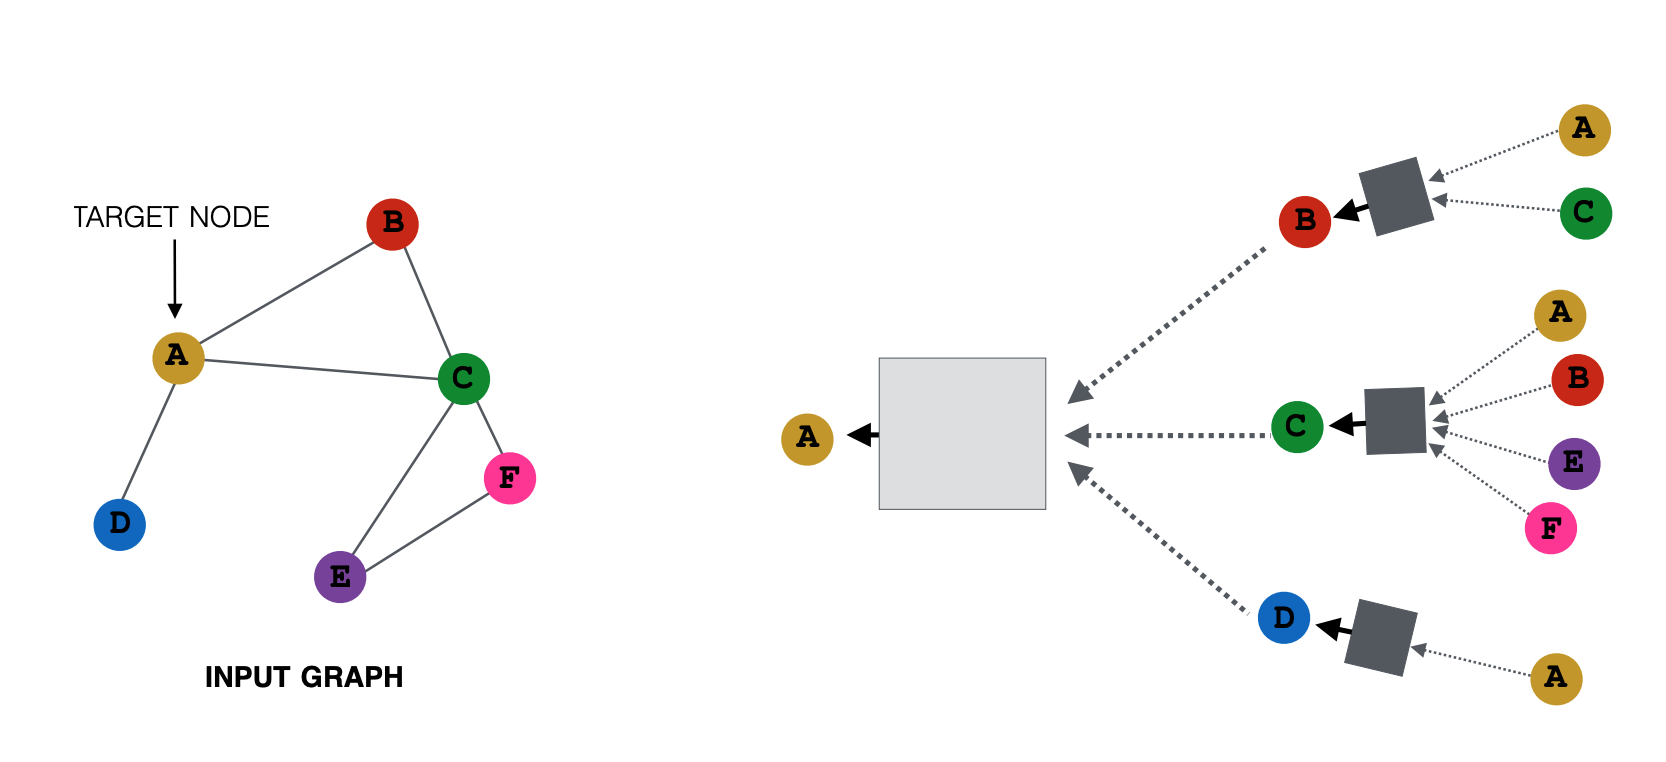
\includegraphics[width=0.8\textwidth]{GNN.png}
		\caption{GNN Structure}
		\cite{leskovec2021lecture}
		\label{fig:GNN_structure}
	\end{figure}

	\noindent The \acs{gnn} structure outlined in figure \ref{fig:GNN_structure} 
	shows an example of a 2-hop or 2 layer \acs{gnn}. The 1-hop convolutional layer 
	considers the neighboring nodes of the target node A. The 2-hop layer 
	considers the neighbors of node A's neighbors. Note, that the target node A 
	is included as an input node in the 2-hop layer. This is reasonable as node 
	A itself is also a neighboring node to its neighbors. Taking the example 
	shown in figure \ref{fig:GNN_structure}, the challenge for the \acs{gnn} is to 
	find node embeddings based on local network neighborhoods \citep{leskovec2021lecture}. 
	The node embeddings at layer 0 correspond to the features of the input nodes 
	where $X = H^{(0)}$. A typical procedure for a \acs{gnn} model is outlined 
	in the pseudo-code shown in algorithm \ref{algo:GNN_struct} 
	\citep{hamilton2017inductive,leskovec2021lecture,you2020design}.	

	\begin{algorithm}[h]
		\scriptsize
		\SetAlgoLined
		\KwIn{Graph $G(V,E)$;}
		\myinput{input features $\{x_v,\forall v \in V\}$;}
		\myinput{node labels $\{y_v, \forall v \in V\}$;}
		\myinput{depth/layers $K$}
		\myinput{Trainable and layer specific parameters $\Theta^{k}$ where
		$W^{k}\in\Theta^{k}, \forall k \in
					\{1,\dots,K\}$;}
		\myinput{non-linearity $\sigma$;}
		\myinput{differentiable aggregator functions $AGGREGATE_{k},\forall k \in
					\{1,\dots,K\}$;}
		\myinput{neighborhood function $\mathcal{N}_{k}:v\rightarrow 2^{V},\forall k \in
					\{1,\dots,K\}$;}
		\myinput{loss function $\mathcal{L}$ such as cross entropy $CE$;}
		\myinput{learning rate $\alpha$}
		\KwOut{Vector representations $z_v, \forall v\in V$}
		\nl Initialize parameters $\Theta$ from $\mathcal{U}$\;
		\nl $h_{v}^{0} = x_{v},\forall v \in V$\\
		\nl \For{Number of epochs}{
		\nl \For{$k=1\dots K$}{
		\nl		\ForAll{$v\in V$}{
		\nl			$h_{\mathcal{N}(v)}^{k} \leftarrow AGGREGATE_k\left(
					{h_{u}^{k-1},\forall u \in\mathcal{N}_{k}(v)}\right)$\;
		\nl			$h_{v}^{k} \leftarrow\sigma \left(W^{k}\cdot 
							CONCAT(h_{v}^{k-1},h_{\mathcal{N}(v)}^{k})\right)$\;
					}		
		\nl		$h_{v}^{k} \leftarrow h_{v}^{k}/\lVert h_{v}^{k}\rVert_{2}$	
   			}
		\nl $z_v = h_{v}^{K},\forall v \in V$\;
		\nl $\mathcal{L}(\Theta)=\sum_{v=1}^{\mid V \mid} CE(y_{v},z_{v})$\;
		\nl $\Theta = \Theta - \alpha\cdot\frac{\partial\mathcal{L}}{\partial\Theta}$
		}
		\caption{Typical GNN Algorithm for Model Training}
		\label{algo:GNN_struct}
	\end{algorithm}

	\noindent Algorithm \ref{algo:GNN_struct} is not meant to be considered as
	a complete overview and should be rather regarded as an example of a typical 
	\acs{gnn} structure. In addition, one should split the data into training-
	and validation sets to ensure a good model fit. \acsp{gnn} are flexible in 
	that a myriad of modifications can be added to the \acs{gnn} layers similar 
	to the possibilities of \acsp{cnn} and \acsp{ann}. The defining features of
	different \acs{gnn} models usually involve the selection of different 
	message passing methods and aggregation strategies. An excellent overview 
	regarding the design space for \acsp{gnn} is provided in the articles by 
	\cite{you2020design} and \cite{zhou2020graph} as a reference. Of course, 
	there are exceptions and alternative procedures exist. The \acs{gnn} methods 
	evaluated in this thesis and most successful \acsp{gnn} however tend to 
	follow a variation of the structure shown in algorithm \ref{algo:GNN_struct}.  \\

	\noindent In terms of interpretation, the output of the first \acs{gnn} 
	layer in figure \ref{fig:GNN_structure} (gray boxes) corresponds to the 
	hidden layer representations of the direct neighbors of the target node A. 
	The output of the final \acs{gnn} layer corresponds to the node embedding 
	$z_{A}$ of the target node A. This should appear familiar when comparing 
	this approach to the \acs{grl} models introduces in the previous section. 
	\acsp{gnn} can indeed be used for unsupervised learning tasks such as 
	learning node embeddings. Good examples for generating node embeddings are 
	shown in the articles regarding \acsp{gcn} by \cite{kipf2016semi} and 
	GraphSage by \cite{hamilton2017inductive}. As shown in algorithm 
	\ref{algo:GNN_struct}, \acsp{gnn} can directly be applied for \acs{ml} tasks 
	such as customer classification. This is where \acsp{gnn} are especially 
	powerful and differ to the \acs{grl} algorithms outlined in the previous 
	section. \acsp{gnn} are flexible tools and can be used in various settings 
	such as \acs{grl}, clustering, classification and link prediction tasks 
	among others \citep{zhou2020graph}. \\

	\noindent Having introduced the general functionality of \acsp{gnn}, the 
	models \ac{gcn} and GraphSage are introduced in detail in the following two 
	sections. 

	\subsubsection{Graph Convolutional Networks}
	
	\noindent The \acf{gcn} was introduced by \cite{kipf2016semi} and makes use 
	of simplified spectral graph convolutions. The author Thomas Kipf 
	\citeyearpar{kipf2016online} provides excellent explanations on his
	website\footnote{Website Thomas Kipf: 
	\url{https://tkipf.github.io/graph-convolutional-networks/}} which is used 
	as inspiration for presenting the theory. As outlined, \acsp{gnn} typically 
	differ with regards to the type of message passing and aggregation strategy 
	applied. \acsp{gcn} make use of the following forward propagation function 
	\citep[p. 2]{kipf2016semi}:

	\begin{equation}
		H^{(l+1)} = \sigma\left(\tilde D^{-\frac{1}{2}}\tilde A \tilde
		D^{-\frac{1}{2}}H^{(l)}W^{(l)}\right)
		\label{eq:GCN}
	\end{equation}
	
	\noindent The variables in equation \ref{eq:GCN} are defined as follows:

	\begin{itemize}
		\setlength\itemsep{0.2em}
		\item $H^{l}\in\mathbb{R}^{N \times D}$ refers to the embedding matrix
			at layer $l$ where $N$ refers to the number of nodes $\mid V \mid$
			and $D$ refers to the number of embedding dimensions. The input
			embedding matrix is set equal to the feature matrix, $H^{(0)}=X$.
		\item $W^{l}$ refers to the trainable and layer specific weight matrix
			for the linear message passing employed in the \acs{gcn} model.
		\item $\tilde A = A + I_N$, where $A$ is the adjacency matrix of the
			input graph $G$. The identity matrix is added so that self-loops
			are considered. This is necessary as the target node of every layer
			is considered in the aggregation process as previously outlined.
		\item $\tilde D_{ii} = \sum_{j}\tilde A_{ij}$ is a diagonal matrix
			containing the degree distributions of the modified adjacency
			matrix $\tilde A$.
		\item $\sigma(\cdot)$ refers to an activation function such as ReLU
			\citep{nair2010rectified} or softmax.
	\end{itemize}

	\noindent To provide a better overview, the compact notation shown in 
	equation \ref{eq:GCN} is expanded in the following equation for one
	\acs{gcn} layer \citep{Dubois2019}:

	\begin{equation}
		h_{ij}^{(l)} = \sigma\left(\sum_{(i,j)\in
		\mathcal{N}(v)}\frac{\tilde a_{ik}h_{kj}^{(l-1)}}{\sqrt{\tilde
d_{k,k}\tilde d_{i,i}}} W^{(l)}\right)
		\label{eq:GCN_expand}
	\end{equation}
	
	\noindent In Equation \ref{eq:GCN_expand} $h_{ij}^{(l)}$ refers to the 
	hidden layer representation of node $i$ at layer $l$ considering the set of
	neighbors $j$. $h_{kj}^{(l-1)}$ corresponds to the hidden layer
	representation of node $k$ at layer $l-1$ which is part of the set of 
	neighbors $j$. In terms of filtering strategy, $(i,j) \in \mathcal{N}(v)$. 
	This means that both set of nodes $i$ and $j$ are neighbors of the target 
	node $v$ at layers $l$ and $(l-1)$ respectively. Linear message
	passing is then performed for every neighbor in $j$ at layer $l-1$. The node 
	in the graph $G$ at position $\tilde a_{ik}$ of the modified adjacency matrix 
	selects the nodes for which a connection between $h_{ij}^{(l)}$ and
	$h_{kj}^{(l-1)}$ exists. The embeddings $h_{kj}^{(l-1)}$ of the selected 
	nodes are normalized by the symmetric degree distributions of the previous 
	hidden layer node $\tilde d_{k,k}$ and the new hidden layer node $\tilde d_{i,i}$.
	Afterwards the normalized embeddings are message passed by multiplying it
	with the shared weight matrix $W^{(l)}$. Lastly, the sum of the received
	messages is taken in terms of aggregation strategy and the resulting
	aggregate is passed through the activation function to yield $h_{ij}^{(l)}$.
	Note, that the aggregation strategy involves taking a weighted sum thanks
	to the symmetric normalization. \\

	\noindent The detailed explanations given above show the procedure for
	one layer of a \acs{gcn}. Returning now to compact notation, this procedure 
	can be expanded for two or more \acs{gcn} layers. First, the notation is 
	further simplified by defining $\hat A = \tilde D^{-\frac{1}{2}}\tilde A \tilde
	D^{-\frac{1}{2}}$. An example of a two layer \acs{gcn} is then given as 
	follows where $Z$ refers to the embedding or output of the target node 
	\citep[p. 3]{kipf2016semi}:

	\begin{equation}
		Z = f(X,A) = \text{softmax}\left(\hat A \;\text{ReLU}\left(\hat A X
		W^{(0)}\right)W^{(1)}\right)
	\label{eq:GCN_forward}
	\end{equation}

	\noindent Finally, the model parameters are updated analogues to the
	procedure outlined in algorithm \ref{algo:GNN_struct}. The main distinctive
	feature for the \acs{gcn} is the differing forward propagation function. 

	\subsubsection{GraphSage}
	
	\noindent This section introduces GraphSage by \cite{hamilton2017inductive} 
	which can be thought of as the inductive counterpart of the \acs{gcn} 
	presented in the previous section. Inductive refers to the capability of 
	not only performing \acs{ml} tasks on the graph used for training but to 
	apply the trained \acs{gnn} model to new and unseen graphs. This is a large 
	leap as \acsp{gcn} for instance can only be used to predict unseen nodes on 
	the graph which was used for training. This is very limiting for the 
	application of \acsp{gcn} in a practical setting. GraphSage overcomes this
	problem by applying different aggregation strategies and sampling the 
	neighborhood $\mathcal{N}(v)$. Specifically, the GraphSage model only 
	considers a fixed number of uniformly random sampled neighbors from 
	$\mathcal{N}(v)$ with depth $K$. A graphical example of this procedure is 
	shown in figure \ref{fig:GraphSage_sample}:

	\begin{figure}[h]
		\centering
		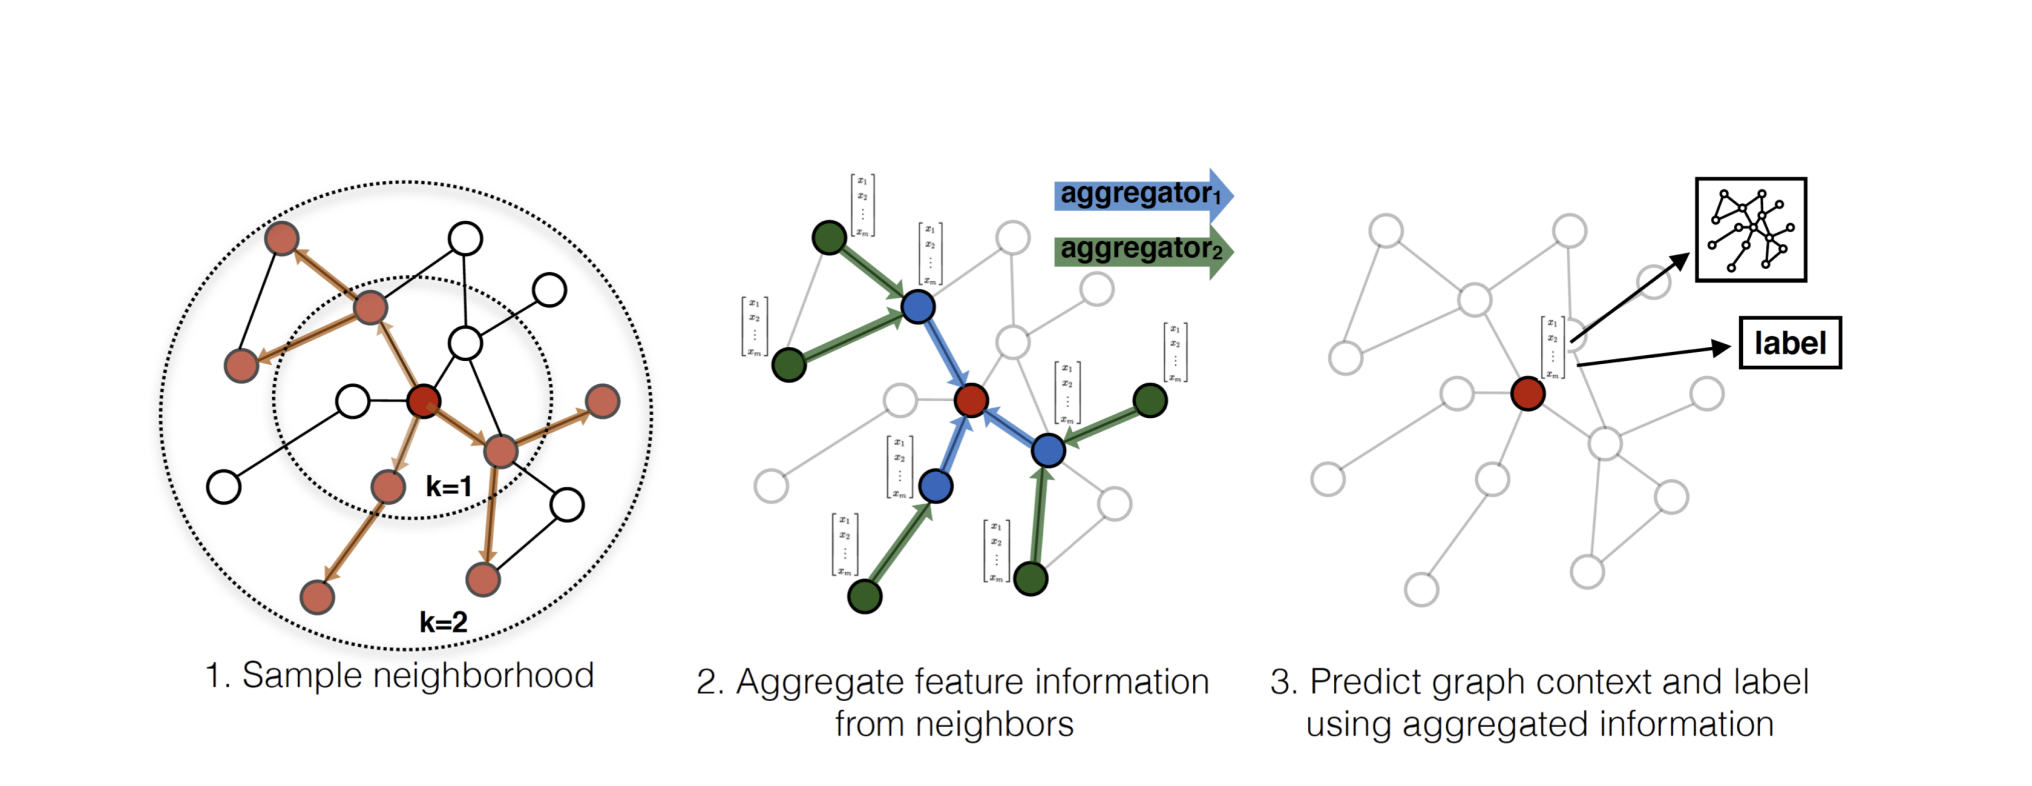
\includegraphics[width=0.8\textwidth]{graphsage.png}
		\caption{GraphSage Sampling}
		\cite[p. 2]{hamilton2017inductive}
		\label{fig:GraphSage_sample}
	\end{figure}

	\noindent The steps shown in figure \ref{fig:GraphSage_sample} are similar
	to the procedures for \acsp{gcn}. The pseudo code for the GraphSage forward 
	propagation function is given in algorithm \ref{algo:GraphSage} 
	\cite[p. 12]{hamilton2017inductive}. \\


	\begin{algorithm}[h]
		\scriptsize
		\SetAlgoLined
		\KwIn{Graph $G(V,E)$;}
		\myinput{input features \{$x_v,\forall v \in \mathcal{B}$\};}
		\myinput{depth $K$;} 
		\myinput{weight matrices $W^{k},\forall k \in\{1,\dots,K\}$;}
		\myinput{non-linearity $\sigma$;}
		\myinput{differentiable aggregator functions $AGGREGATE_k,\forall k \in
					\{1,\dots,K\}$;}
		\myinput{neighborhood sampling functions, $\mathcal{N}_k:v\rightarrow
					2^{v},\forall k \in \{1,\dots,K\}$}
		\KwOut{Vector representations $z_v$ for all $v\in\mathcal{B}$}
		\nl $\mathcal{B}^{K}\in\mathcal{B}$\\
		\nl \For{$k=K\dots 1$}{
		\nl		$\mathcal{B}^{k-1}\leftarrow\mathcal{B}^{k}$\\
		\nl		\For{$u\in\mathcal{B}^{k}$}{
		\nl			$\mathcal{B}^{k-1}\leftarrow\mathcal{B}^{k-1}\cup\mathcal{N}_{k}(u)$
					}
				}
		\nl $h_{u}^{0}\leftarrow x_{v},\forall v \in \mathcal{B}^{0}$\\
		\nl \For{$k=1\dots K$}{
		\nl		\For{$u\in\mathcal{B}^{k}$}{
		\nl			$h_{\mathcal{N}(u)}^{k}\leftarrow
					AGGREGATE_k(\{h_{u'}^{k-1},\forall u'\in \mathcal{N}_{k}(u)\})$\;
		\nl			$h_{u}^{k}\leftarrow\sigma\left(W^{k}\cdot
					CONCAT(h_{u}^{k-1},h_{\mathcal{N}(u)}^{k})\right)$\;
		\nl			$h_{u}^{k} \leftarrow h_{u}^{k}/\lVert
					h_{u}^{k}\rVert_{2}$		
				}		
			}
		\nl $z_v \leftarrow h_{u}^{K},\forall u \in \mathcal{B}$
		\caption{GraphSage Minibatch Forward Propagation Algorithm}
		\label{algo:GraphSage}
	\end{algorithm}
	
	\noindent Note that algorithm \ref{algo:GraphSage} assumes that the
	parameters of the aggregator functions and the weight matrices $W$
	are known. Algorithm \ref{algo:GraphSage} thus shows the forward
	propagation of a trained GraphSage model. The model is trained by
	optimizing the model parameters using mini-batch training for a specified 
	number of epochs. The training procedure can be implemented by using an
	adaptation of the general procedure shown in algorithm \ref{algo:GNN_struct}. 
	Note, that the parameters of the aggregation functions and the weight 
	matrices $W$ are all layer specific elements of $\Theta$ in algorithm 
	\ref{algo:GNN_struct}. For algorithm \ref{algo:GraphSage}, $\mathcal{B}$ 
	refers to the mini-batches of vertices taken from the set of vertices $V$ 
	of the graph $G(V,E)$. \\

	\noindent There are three aggregator types proposed for GraphSage
	\citep[p. 5-6]{hamilton2017inductive}:

	\begin{enumerate}
		\setlength\itemsep{0.2em}
		\item Mean aggregation
		\item Max-pooling
		\item Long short-term memory (\acs{lstm}) aggregation
	\end{enumerate}

	\noindent The three proposed aggregation strategies are briefly introduced
	as follows:

	\paragraph{Mean Aggregation} \mbox{}\\
	\noindent This type of aggregation is similar to the \acs{gcn} and takes the
	average of the received messages from the message passing procedure. The 
	difference to \acs{gcn} is that mean aggregation does not rely on the full 
	graph Laplacian and makes use of a slightly different normalization approach. 
	The aggregation process differs to the one shown in algorithm 
	\ref{algo:GraphSage} and replaces the procedures in line 9 and 10 with 
	\citep[p. 5]{hamilton2017inductive}:

	\begin{equation}
		h_{v}^{k} \leftarrow \sigma\left(W\cdot
		\text{MEAN}(\{h_{v}^{k-1}\}\cup\{h_{u}^{k-1},\forall u \in \mathcal{N}(v)\})\right)
	\end{equation}

	\paragraph{Max-Pooling Aggregation} \mbox{}\\
	\noindent Max-Pooling aggregation refers to the application of an 
	element-wise $\max$ operator. This means that of the neighbors, only the 
	largest element-wise features are considered. More formally, max-pooling 
	aggregation is defined as follows and is used for the aggregation shown in 
	line 9 of algorithm \ref{algo:GraphSage} \citep[p. 6]{hamilton2017inductive}:

	\begin{equation}
		AGGREGATE_{k}^{pool} = \max\left(\sigma(\{W_{pool}h_{u_{i}}^{k} +
		b),\forall u_{i} \in \mathcal{N}(v)\}\right)
	\end{equation}

	\noindent Note, that $W_{pool}$ refers to a separate weight matrix for the
	one layer message passing of the max-pooling aggregation. In principle, an 
	arbitrary number of layers could be added for max-pooling. The authors 
	\cite[p. 6]{hamilton2017inductive} however focus on the case with one layer. 
	This approach is kept as it yielded good results. The parameters of 
	max-pooling are learned analogues to the other GraphSage model parameters. \\ 

	\paragraph{LSTM Aggregation} \mbox{}\\
	\noindent \Acf{lstm} is the last aggregation strategy 
	proposed for GraphSage and uses the \acs{lstm} \acf{rnn} first introduced by
	\cite{hochreiter1997long} as an aggregation strategy. \acsp{lstm} are not
	permutation invariant which is a requirement for the aggregation strategy.
	The authors propose using a random permutation of the set of node neighbors 
	to counter this problem \citep[p. 5]{hamilton2017inductive}. The \acs{lstm}
	parameters are trained along with the other GraphSage model parameters.  

	\section{Graph Generation}
	\label{section:theory_graphgen} 

	This section introduces the \acf{mag} model by \cite{kim2012multiplicative}. 
	This model is used to generate semi-synthetic graphs from feature data as 
	mentioned in the introduction. Originally, the MAG model was introduced for 
	the purpose of generating realistic graphs from feature data and to show that 
	the resulting graph can obey properties of real-world networks. To show this, 
	\citeauthor{kim2012multiplicative} generated random feature data for which 
	the model parameters were set in such a manner, that the resulting graph 
	adheres to a set of real network properties. These network properties 
	include the emergence of a giant connected component and a power-law or 
	$\log$-normal degree distribution among others 
	\citep[p. 113]{kim2012multiplicative}. While the creation of a graph which 
	follows real-world network properties would be desirable, it is not the 
	primary target for this thesis. The main goal of the semi-synthetic graph 
	generation is to create a graph that provides useful additional information, 
	which can be exploited using \acs{gml}. The \acs{mag} model is flexible in 
	this sense, that it can create graphs which are not constrained to adhere to 
	a specific set of network properties. Lastly, 
	\citeauthor{kim2012multiplicative} 
	\citeyearpar[p. 138-139]{kim2012multiplicative} present model parameters 
	which generate graphs that follow real-world network properties. These model 
	parameters can however not be adopted for the task at hand. The parameters 
	were created for a somewhat simpler task which "only" involved randomly 
	generated feature data. These randomly generated features do not correspond
	to any specific features. For that reason, the model parameters can be
	chosen freely such that the generated network follows real world network
	properties. The aim of \citeauthor{kim2012multiplicative} was primarily to
	create random graphs that can adhere to said network properties. For this
	thesis, the same MAG model will applied using real feature data. This makes
	the task of defining the model parameters more difficult as they cannot be
	freely assigned. In addition, the generated graph will be used for \acs{ml} 
	which is not an application the authors had considered. In this regard the 
	reason and aim for using the \acs{mag} model differs for this thesis 
	compared to the original paper. \\

	\noindent The starting point of the \acs{mag} model is a matrix of feature 
	data, $X^{N \times F}$, where $N$ refers to the number of observations 
	and $F$ to the number of features. \citeauthor{kim2012multiplicative} refer 
	to feature data as attributes and they use the terms interchangeably. For this 
	thesis a distinction is made, where features correspond to the full set of 
	feature data and attributes refer to the $K$ number of features used for 
	generating the graph, $G(V,E)$. The attribute data, 
	$B^{N \times K} \subseteq X^{N \times F}$, is therefore a subset of the 
	feature data. As a selection criterion, attribute data must be of such a 
	manner that reasonable link-affinity matrices, $\Theta_{i}$, can be 
	defined. In addition, attribute data must be discrete. For practical
	reasons, the cardinality of the attributes should not be too large.
	Attributes such as age might have to be discretized into 4 or 5 discrete
	age categories. The link-affinity matrix $\Theta_{i}$ is a matrix
	containing probabilities which are used to estimate the probability of two 
	observations in the dataset $(u,v)$ to form a connection. More specifically, 
	the probability for a connection is calculated given the attributes $a_i$ of 
	observation $u$ and $v$ where $(a_{i}(u),a_{i}(v))\in B$. For example, a 
	reasonable assumption could be to assume, that people which are of the same 
	age group, are more likely to be similar and thus form a connection 
	compared to people which are not of the same age group. Another example for 
	this could be gender in terms of biological sex which is a classical binary 
	setting for a link-affinity matrix. Examples of binary attribute 
	link-affinity matrices $\Theta_i$ are given in 
	figure \ref{fig:link-affinity}.

	\begin{figure}[h]
		\centering
		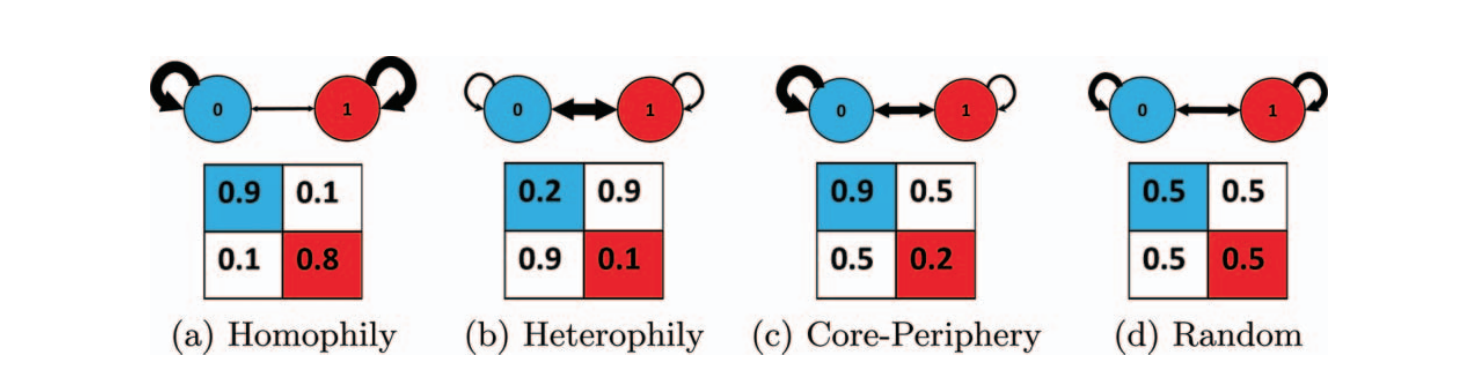
\includegraphics[width=0.9\textwidth]{affinity_matrices.png}
		\caption{Attribute Link-Affinities}
		\cite[p. 118]{kim2012multiplicative}
		\label{fig:link-affinity}
	\end{figure}

	\noindent Figure \ref{fig:link-affinity} shows 4 types of link-affinity
	matrices depending on the type of relationship one wants to model. Homophily 
	refers to love of the same which would make a connection between two
	observations more likely if they have the same attributes. Similarly,
	Heterophily refers to the love of the different where observations which do 
	not have the same attributes are more likely form a connection. 
	Core-periphery is a special case which can be used to generate realistic 
	social-networks in terms of network properties 
	\citep[p. 139]{kim2012multiplicative}. As an example, an attribute could
	indicate whether a person is a member of the local football club. In a
	core-periphery setting, members of the local football club are very likely
	to be connected, while non-members have a significantly lower probability
	of forming a connection. Lastly, random graphs can be generated by setting the
	link-affinity probabilities to 0.5. Given the type of attributes available
	in the data sets, graphs will be generated using homophily structures. The 
	attribute link-affinity matrices $\Theta_i$ are defined for every attribute 
	and can be set for an arbitrary size of categories within an attribute. 
	More formally for each observation $u \in B$ with $K$ categorical attributes 
	of cardinality $d_i$ for $i = 1,2,\dots,K$ and corresponding link-affinity 
	matrices $\Theta_{i}^{d_{i} \times d_{i}}$ for $i=1,2,\dots,K$, the probability 
	$P[u,v]$ of a connection between observations $(u,v)$ is defined as 
	\citep[p. 119]{kim2012multiplicative}:

	\begin{equation}
		P[u,v] = \prod_{i=1}^{K}\Theta_{i}\left[a_{i}(u),a_i(v)\right]
		\label{eq:MAG}
	\end{equation}

	\noindent In equation \ref{eq:MAG}, $a_{i}(u)$ refers to the value of the 
	$i$th attribute of observation $u$. A schematic representation of the 
	procedure for a binary link-affinity matrix is shown in figure \ref{fig:MAG}.

	\begin{figure}[h]
		\centering
		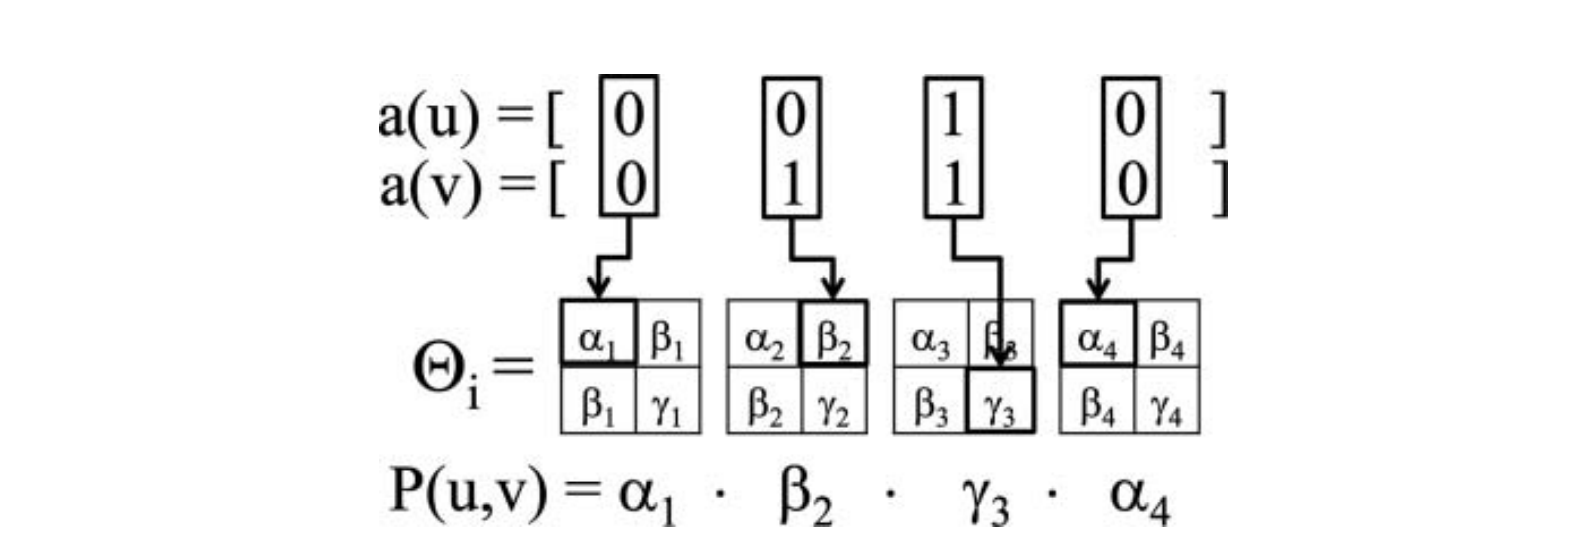
\includegraphics[width=0.8\textwidth]{MAG.png}
		\caption{Schematic Representation of the 
			Multiplicative Attribute Graphs (MAG) Model}
		\cite[p. 120]{kim2012multiplicative}
		\label{fig:MAG}
	\end{figure}
	
	\begin{algorithm}[h]
		\scriptsize
		\SetAlgoLined
		\KwIn{graph node-attribute generation matrix $B^{N \times K}$, where 
			$B\subseteq X^{N \times F}$;}
		\myinput{node attribute vector $a_i$ with
			cardinalities $d_i$ for $i=1,2,\dots,K$;}
		\myinput{link affinity matrices $\Theta_{i}^{d_i \times d_i}$, for $i= 1,2,\dots,K$;}
		\KwOut{adjacency Matrix $A^{N\times N}$ for Graph $G(V,E)$} 
		\nl $B^{K \times N} = B^{T}$ \\
		\nl \For{$j = 1,2,\dots,N$}{
		\nl	$u = B[:,j]$\\
		\nl		\For{$k = 1,2,\dots,N$}{
		\nl			$v = B[:,k]$\\
		\nl			\For{$i = 1,2,\dots,K$}{
		\nl				$P_{j,k} = \prod_{i=1}^{K}\Theta_{i}[a_{i}(u),a_i(v)]$
						}
				}
			}
		\nl $U^{N \times N} = uppertriangular(P)$ with $diag(U)=0$\\
		\nl \For{$i=1,2,\dots,N$}{
		\nl		\For{$j=1,2,\dots,N$}{
		\nl			\If{$U_{i,j} > \mathcal{U}(0,1)$}{
		\nl				$\hat A_{i,j} = 1$} 
		\nl			\Else{$\hat A_{i,j} = 0$}
				}
			}
		\nl $A = \hat A + \hat A^{T}$
		\caption{Multiplicative Attribute Graph Model}
		\label{algo:MAG}
	\end{algorithm}

	\noindent The pseudo-code of the \acs{mag} model is depicted in algorithm 
	\ref{algo:MAG} and generates the adjacency matrix $A$ which is then used 
	for constructing the graph $G(V,E)$. The observations of the feature data 
	$X$ which contains the attributes are used as inputs and correspond to the 
	nodes in the resulting graph. More precisely, the order of the generated 
	adjacency matrix $A$, corresponds to the ordering of the feature matrix $X$. 
	Therefore the features can be assigned to the nodes of the generated graph. 
	The procedure outlined in algorithm \ref{algo:MAG} can be summarized with 
	the following sequential steps:

	\begin{enumerate}
		\item Calculate the connection probabilities $P$ between every 
			observation in the attribute matrix $B$ using equation \ref{eq:MAG}. 
		\item As only undirected graphs are considered, the upper triangular
			matrix $U$ of $P$ is taken where the $diag(U) = 0$. The diagonal of
			$U$ is set to 0 to exclude self-loops.
		\item For every element in $U$, draw a random number form a standard
			uniform distribution $\mathcal{U}(0,1)$. If the connection
			probability $P_{u,v}>\mathcal{U}(0,1)$, a 1 in the
			preliminary adjacency matrix $\hat A_{u,v}$ is recorded.
			Otherwise a 0 is recorded.
		\item The preliminary adjacency matrix $\hat A$ is an upper triangular
			matrix with $diag(\hat A) = 0$ and all elements in the lower
			triangular also being equal to 0. As the target is to create an
			undirected graph, the corresponding adjacency matrix is symmetric
			which is why the final adjacency matrix can be created using 
			$A = \hat A + \hat A^{T}$. 
	\end{enumerate}
 
